\documentclass{acsman}
\usepackage{float}
\usepackage[dvipdfmx]{graphicx}
\usepackage{url}
\usepackage{amsmath}
\usepackage{subfigure}
\usepackage{titlesec}
\usepackage{tabularx}
\usepackage{booktabs}
\usepackage{multirow}
    \newcolumntype{C}{>{\centering\arraybackslash}X}
    \newcolumntype{L}{>{\raggedright\arraybackslash}X}
    \newcolumntype{R}{>{\raggedleft\arraybackslash}X}



\pagestyle{myheadings}

\setcounter{page}{
%%%   ページ数の設定 (Page number)   %%%
1
%%%%%%%%%%%%%%%%%%%%%%%%%%%%%%%%%%%%%%%%
}

\begin{document}
\noindent
\twocolumn[
\Large
\begin{flushright}
\fbox{学外秘}
\end{flushright}



\begin{center}
{\bf
%%%   題目 (Title)   %%%
Watercolor Image Generation Based on Diffusion Model
%%%%%%%%%%%%%%%%%%%%%%%%
}
\end{center}
\normalsize
\vspace{\baselineskip}
\normalsize
\begin{tabular}{@{}p{18zw}@{}p{12zw}@{}}
\centering{
\small
%%%   研究科 (Faculty or Graduate Course)   %%%
広島大学大学院先進理工系科学研究科
%%%%%%%%%%%%%%%%%%%%%%%%%%%%%%%%%%%%%%%%%%%%%%%
}
&
\hfil
{\small
%%%   専攻 (Course or Major)   %%%
情報科学プログラム
%%%%%%%%%%%%%%%%%%%%%%%%%%%%%%%%%%
}
\hfil \\
\centering{
\small
%%%   学生番号 (Number)  %%%
M225163					%←ここに学生番号を書く.
%%%%%%%%%%%%%%%%%%%%%%%%%%%%
}
&
\hfil
{\small
%%%   氏名 (Name)   %%%
張 邦林				%←ここに名前を書く.
%%%%%%%%%%%%%%%%%%%%%%%
}\hfil
\end{tabular}
\ \
\begin{tabular}{@{}l@{}}
{\small
指導教官:
%%%   指導教官 (Instructors)   %%%
中野 浩嗣
%%%%%%%%%%%%%%%%%%%%%%%%%%%%%%%%%%
}\\
{\small
所  属:
%%%   所属 (Affiliation)   %%%
コンピュータ・システム研究室
%%%%%%%%%%%%%%%%%%%%%%%%%%%%%%
}
\end{tabular} \par\noindent
\normalsize
\vspace{2\baselineskip}
]
%%%  概要 (Abstract)   %%%
\begin{abstract}
With the development of deep learning, the application of deep learning in image generation is becoming more and more widespread. Especially the generation of images in various special styles, such as oil painting style, sketch style and watercolor style. However, existing research on watercolor style image generation is often achieved by style conversion, which limits the creative ability of the model. At the same time, the models do not simulate the watercolor effect well.

In this paper, in order to solve the above problems. Firstly, a high-quality watercolor image dataset is produced and used for model training. In order to achieve the purpose of generating high quality watercolor images. Starting from Vision Transformer and diffusion model, this study abandons the U-Net structure commonly used in diffusion model and redesigns the network structure of diffusion model based on Vision Transformer. Compared with the existing model, the quality of watercolor image generation is improved.
\end{abstract}

%%%  本文 (Text)   %%%

\section{Introduction}
The rapid development of deep learning techniques has not only led to remarkable achievements in the traditional fields of computer vision and natural language processing, but has also demonstrated its potential in the creation of art. One notable application is the use of deep learning to generate watercolor images, which provides a whole new dimension to digital art. Watercolors are known for their distinctive brushstrokes, soft color transitions, and unique style of the artist, and deep learning techniques are able to simulate and reproduce this traditional art form in an unprecedented way. However, due to the characteristics of watercolor images, popular deep learning generation models often fail to achieve satisfactory results. This has driven the development of specialized generative network architectures for watercolor image generation. to meet the needs of art creation, film and animation production or customized product design. In this study, in order to achieve high quality watercolor image generation. A high quality watercolor image dataset was produced and a new watercolor image generation network was designed for this task.

With the rapid development of deep learning techniques, image generation tasks are gradually categorized into two main research areas. As shown in Figure \ref{fig:intro} , label-based image generation and image generation based on input images \cite{isola2017image}. Most of the deep learning generation models on watercolor images before this are graph-generated tasks, and very few of them are based on label generation \cite{wang2023stroke}. This does not allow the model to be innovative and stochastic, whereas models for artistic creation like watercolor images. It is in line with the demand to make the model appear artistic and abstract generation appropriately. Therefore, this study revolves around label based generation of watercolor images.

\begin{figure}[h]
    \centering
    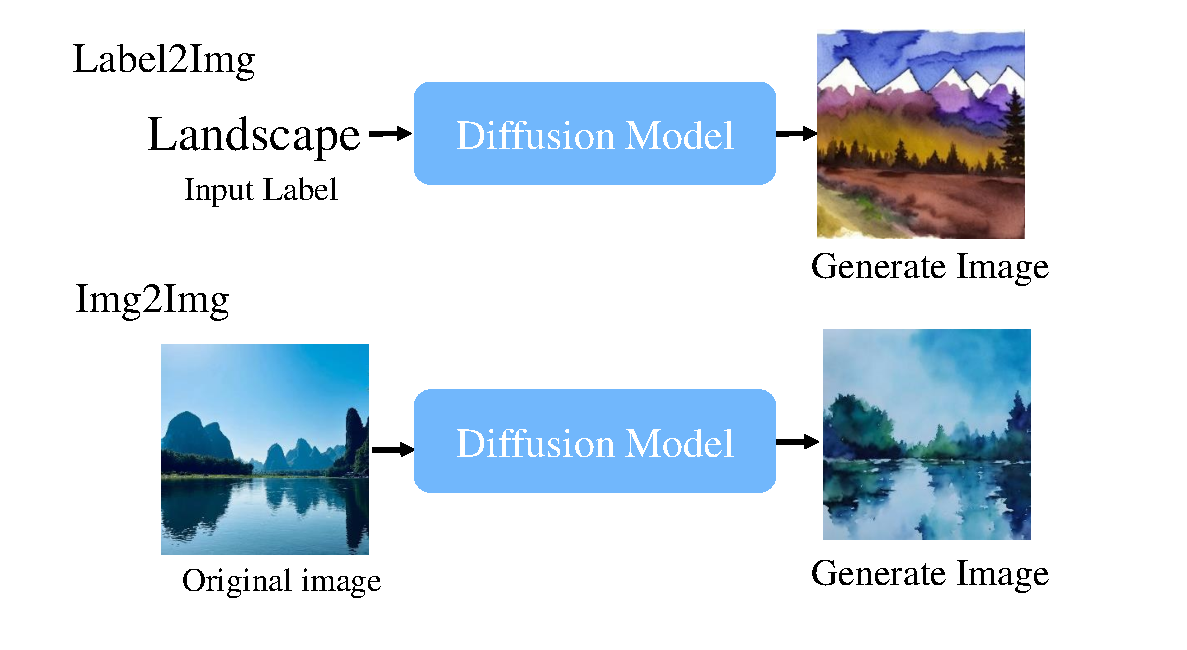
\includegraphics[width=8cm]{image/intro.pdf}
    \caption{Different image generation methods}
    \label{fig:intro}
\end{figure}

Also, the network structure used is categorized according to the network structure used. The current mainstream ones are adversarial generative networks and diffusion models. Adversarial generative network \cite{goodfellow2020generative} as the most widely used generative model, but there are many problems such as pattern collapse, it is difficult to generate high-quality images. Therefore, this paper abandons the use of adversarial generation network and uses the diffusion model with stable effect.

In the diffusion model U-Net is widely used, U-Net is a network structure proposed in 2015, which was first used for image segmentation tasks \cite{ho2020denoising}\cite{ronneberger2015u}\cite{rombach2022high}. Due to its excellent performance it was soon ported to other domains. However, when the diffusion model with U-Net structure is used to generate watercolor images, problems such as unclear targets occur. So in this paper, in order to improve the generation of watercolor images, we give up the use of U-Net structure, and design the diffusion model backbone network structure from scratch based on the inspiration of Vision Transformer and other models \cite{dosovitskiy2020image}, in order to achieve the purpose of generating high-quality watercolor images.The paper is organized as follows, section 2 begins with a description of the related work. Section 3 describes the dataset used and the methodology used for its collection. Then, Section 4 describes the methodology proposed in this paper. Finally,  results and conclusions.

\section{Related Work}\label{sec:related work}
\subsection{Vision Transformer(ViT)}
Vision Transformer model \cite{dosovitskiy2020image} architecture typically consists of components such as a linear embedding layer, a self-attention layer, a fully-connected feed-forward network layer, and residual connectivity with layer normalization.

Unlike traditional convolution-based approaches, Vision Transformer proposes a new paradigm for visual processing. The image is segmented into a series of fixed-size blocks, and the relationships between the blocks are established through a multi-head attention mechanism. The core of this idea is to view the image as a sequence rather than a grid, allowing the model to better capture global information while reducing the number of parameters and computational complexity.

The multi-head attention mechanism allows the model to focus on information at different locations in parallel, effectively dealing with long-range dependencies. ViT performs well when dealing with large-scale image data, with a relatively small number of parameters compared to traditional convolutional networks, providing better scalability. Since it does not rely on a fixed local receptive field, ViT is more flexible in handling images of different sizes and application areas.

\subsection{Diffusion Probabilistic Models(DDPM)}
The key idea of Diffusion Probabilistic Models \cite{ho2020denoising} is to gradually evolve a simple noise distribution into a target data distribution through a diffusion process.Specifically, the basic assumption of Diffusion Probabilistic Models is that an initial simple probability distribution, usually Gaussian (Gaussian noise image). It gradually evolves into a target data distribution (Generated image) through a series of probabilistic diffusion steps. This process can be accomplished by iteratively applying the diffusion operation. 
\begin{figure}[h]
    \centering
    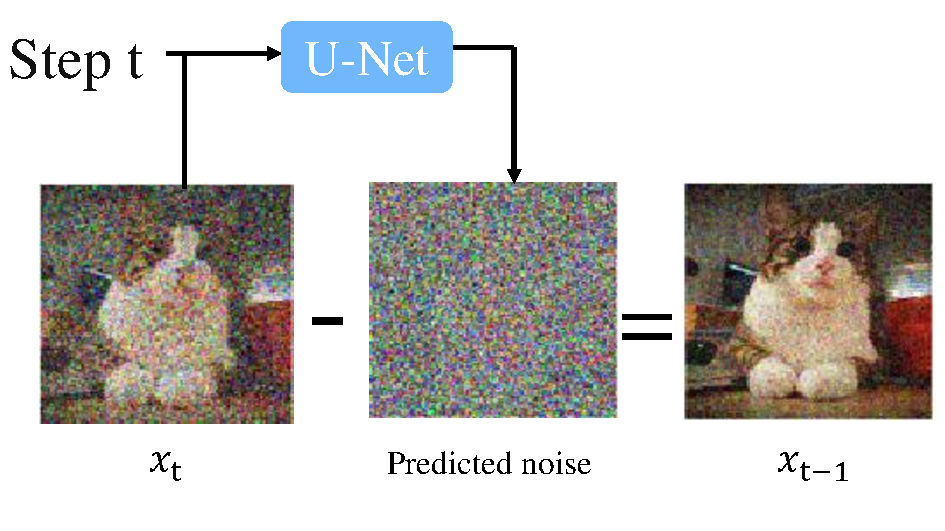
\includegraphics[width=8cm]{image/DDPM.pdf}
    \caption{DDPM single execution process}
    \label{fig:DDPM}
\end{figure}

As shown in Figure \ref{fig:DDPM}, at each step, by removing some of the noise, the current distribution evolves into the distribution for the next step. By performing multiple steps, the model learns how to generate samples (Generated image) that match the target data distribution from a simple distribution (Gaussian noise image)As shown in Figure \ref{fig:DDPM1}.
\begin{figure}[h]
    \centering
    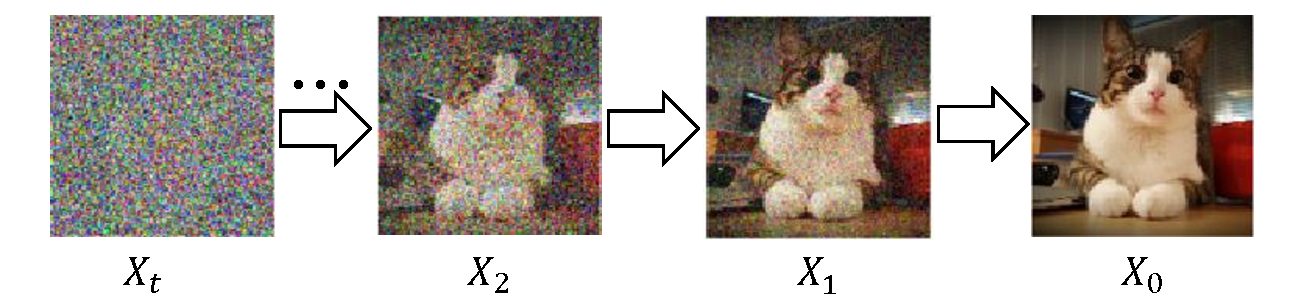
\includegraphics[width=8cm]{image/DDPM1.pdf}
    \caption{Image generation process for DDPM}
    \label{fig:DDPM1}
\end{figure}

One advantage of Diffusion Probabilistic Models is that they do not require adversarial training like GANs or an inference process like VAEs. This makes such models easier to train in some cases.
\subsection{U-Net Used in Diffusion Model}
U-Net is a convolutional neural network architecture for image segmentation tasks \cite{ronneberger2015u}.U-Net is inspired by the structure of the human eye and has two main parts, the encoder (down-sampling path) and the decoder (up-sampling path), and introduces jump connections. The encoder captures local features of the image by stacking convolutional and pooling layers to gradually reduce the spatial dimension of the input image. The decoder gradually recovers the spatial resolution of the image by upsampling and convolutional layers while incorporating feature information from the encoder. This allows the network to fuse different levels of feature information for better detail preservation and improved segmentation performance.Due to the excellent performance of U-Net, it is rapidly being used in various fields.
From the MLP used by Sohl-Dickstein in 2015, to Song Yang in 2019 in the first use of U-Net to construct a diffusion model, many subsequent works such as DDPM , ADM , Imagen and so on have made a series of improvements to U-Net. At present, most papers on diffusion probability modeling still use U-Net as the backbone network.

Diffusion probabilistic models have made many advances in probabilistic modeling since they were first proposed in 2015, and many improvements have been made to their backbone networks, from the MLP used by Jascha in 2015 \cite{sohl2015deep}, to Song Yang's work in 2019 when he first constructed a diffusion model using the U-Net \cite{song2019generative}, and a series of improvements to the U-Net by subsequent works such as the DDPM \cite{ho2020denoising}, and the Imagen \cite{saharia2022photorealistic}. Imagen and many other works have made a series of improvements to U-Net. At present, most papers on diffusion probability modeling still use U-Net as the backbone network.

At the same time, the Transformer architecture has demonstrated high performance in natural language processing, as well as in computer vision, achieving excellent results on a variety of tasks.
\section{Datasets}\label{sec:dataset}
Since there is no publicly available dataset of watercolor images, the first step in this study was to collect a large number of high-quality watercolor images. Therefore, a GPU-based watercolor style conversion program was used to convert images from 30 categories in the ImageNet dataset to watercolor style.

\subsection{ImageNet Datasets}
The ImageNet dataset is a large-scale image dataset originally created by Fei-Fei Li of Stanford University and others \cite{deng2009imagenet}.ImageNet contains more than a million high-resolution images covering a thousand different categories. Each category typically contains hundreds to thousands of images. Each image is accompanied by detailed labeling information, including the categories of objects contained in the image. This is very important for this study, which eliminates the need to spend effort on labeling watercolor images.

\begin{figure}[h]
    \centering
    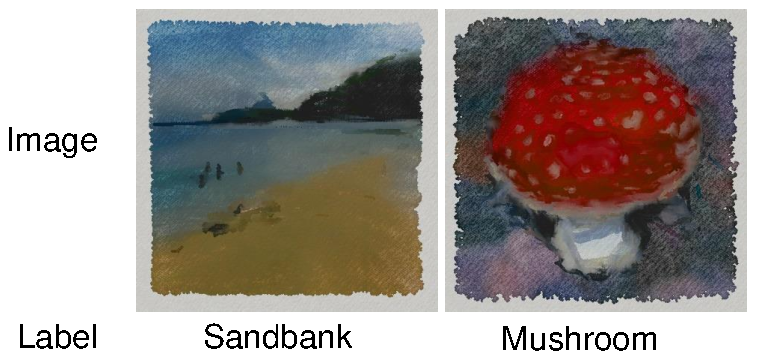
\includegraphics[width=7cm]{image/dataset.pdf}
    \caption{Example of the watercolored ImageNet dataset}
    \label{fig:dataset}
\end{figure}

\subsection{Dataset collection method}
A GPU-based watercolor style conversion method \cite{huang2021gpu}, this method converts the style of an input image into a watercolor image. The study used a stroke-based rendering method that uses physical watercolor simulations to generate stretchable, high-quality watercolor images. However, the study requires input high-resolution images.The original 256$\times$256 resolution images of the ImageNet dataset suffer from problems such as pattern collapse when watercolor style transformation is performed. Therefore, the watercoloring of ImageNet dataset images is divided into two steps, firstly, the dataset images are upgraded to 512$\times$512 resolution, and then the images are watercolored. As shown in Figure \ref{fig:gpu}.

\begin{figure}[h]
    \centering
    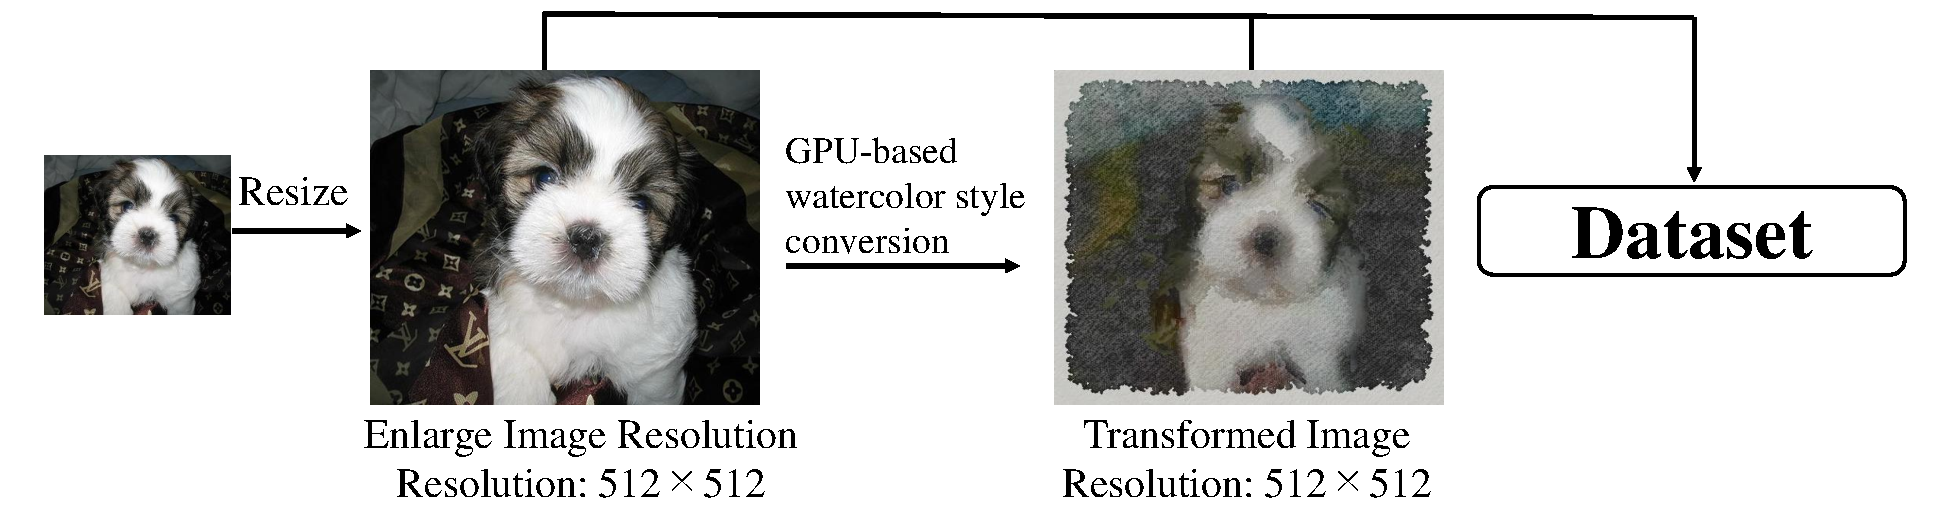
\includegraphics[width=8cm]{image/gpu.pdf}
    \caption{The process of watercoloring ImageNet image}
    \label{fig:gpu}
\end{figure}

Through the above method, a total of 30 categories with a total of 24,550 watercolor images are collected for model training. Figure \ref{fig:dataset} shows an example of the watercolored ImageNet dataset.
\begin{figure}[h]
    \centering
    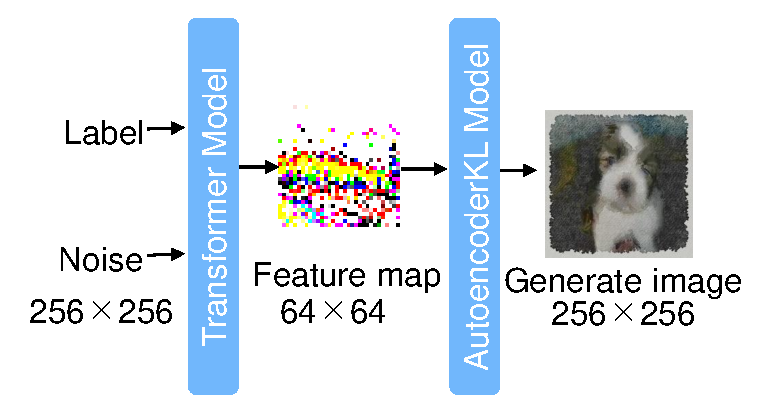
\includegraphics[width=7cm]{image/pm.pdf}
    \caption{Model inference process}
    \label{fig:PM}
\end{figure}
\begin{figure*}[tbp]
    \centering
    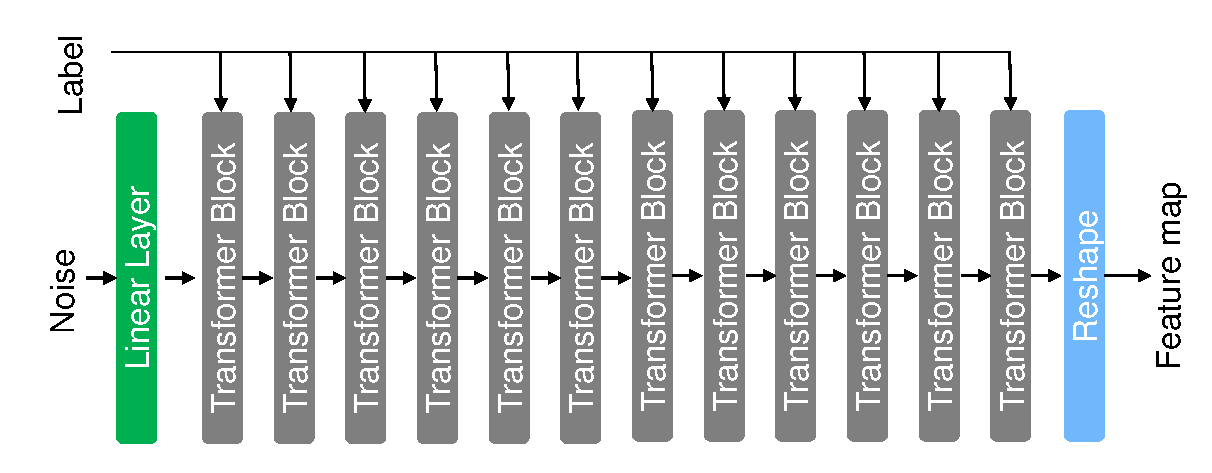
\includegraphics[width=15cm]{image/traM.pdf}
    \caption{Transformer model structure}
    \label{fig:traM}
\end{figure*}
\section{Proposed Method}\label{sec:method}
Previously, most watercolor image generation studies were based on GAN models.In this study, based on the diffusion model and referring to Vision Transformer, the common U-Net is abandoned and the basic modules of the network are redesigned. The model in this study is not end-to-end, but consists of two networks, AutoencoderKL model and transformer model.In the inference process of the model, the Transformer model first generates a feature map based on the input labels. Then, the AutoencoderKL model transforms this feature map into a watercolor image. As shown in Figure \ref{fig:PM}.

\subsection{AutoencoderKL Model}
The variational autoencoder model with KL loss was introduced in Auto-Encoding Variational Bayes by Diederik P. Kingma and Max Welling \cite{kingma2013auto}. The model is used in Diffusers to encode images into latents and to decode latent representations into images.

The original diffusion model is generated at the pixel level. This means that the final image is generated directly from the noise. There are two problems with this scheme: one, the pixel level generation is computationally expensive; and two, the generated image is very cluttered and does not allow for the generation of an image with a specific target.
The AutoencoderKL model is used to solve the above problems. It consists of two parts: encoder and decoder. It is pre-trained and does not need to be re-trained. The introduction of the AutoencoderKL model transforms the transformer model into a feature map generation model. This greatly reduces the computational complexity and improves the controllability of the generation.

Specifically, AutoencoderKL can be used in conjunction with the diffusion model in two ways. Model Training: Use the encoder to extract a feature map from the image and train with that feature map. Model generation: the feature map generated by the transformer is reduced to the image using the decoder.

\subsection{Transformer model}
The design of the Transformer Block follows the basic vision transformer design \cite{dosovitskiy2020image}. The difference is that this study does not place the MLP layer after the attention layer, but uses the MLP layer to process the input labeling information for better control. The number of attentions layers is also increased to enhance the model representational capability. Compared to U-net, the attention mechanism of transformer series can learn the global features of the image better, which has a crucial effect on the generation of watercolor images. Because for watercolor images, what is more important is the overall style of the image rather than the objects within the image.
\begin{figure}[h]
    \centering
    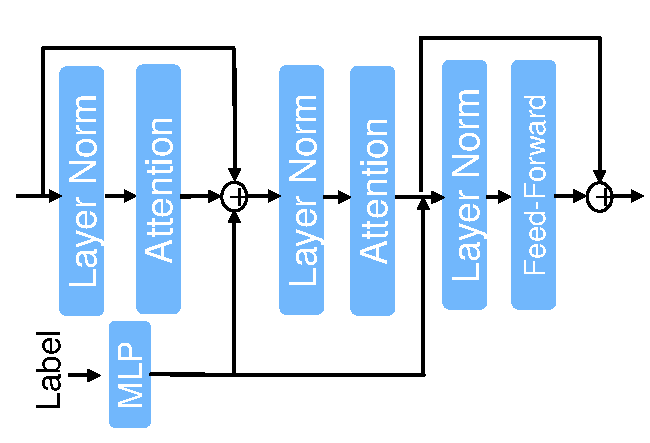
\includegraphics[width=7cm]{image/traB.pdf}
    \caption{Transformer block structure}
    \label{fig:traB}
\end{figure}

\begin{figure*}[tbp]
    \centering
    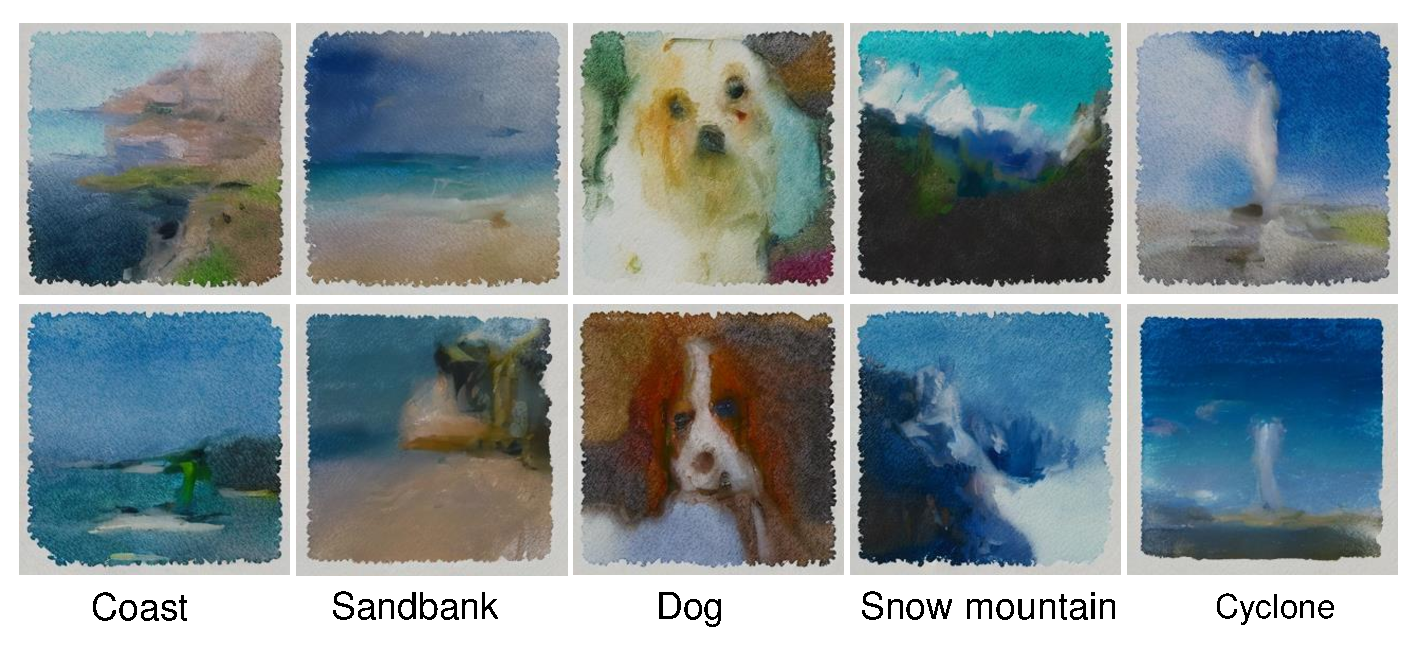
\includegraphics[width=15cm]{image/eva1.pdf}
    \caption{More categories of generated results}
    \label{fig:eva1}
\end{figure*}
The Transformer model consists of a stack of Transformer blocks. In the network designed in this paper, a total of 12 Transformer blocks are used. in order to enable the model to better distinguish between individual labels and induce the model to differentiate the output. The label information is fed into each Transformer block so that the model gets more label information to guide the output. At the same time, in order to reduce the increase in computation brought about by the increase in Transformer blocks, a linear structure is used in the stacking method.

\section{Results}\label{sec:result}
\subsection{Train Details}
To train this model, NVIDIA RTX A6000$\times$2 was used. and the batch size was set to 16, the learning rate was 1e-4, and the optimizer was selected as AdamW. A total of 1500 epochs were trained, and checkpoints were saved at every 300 epochs.
\begin{figure}[h]
    \centering
    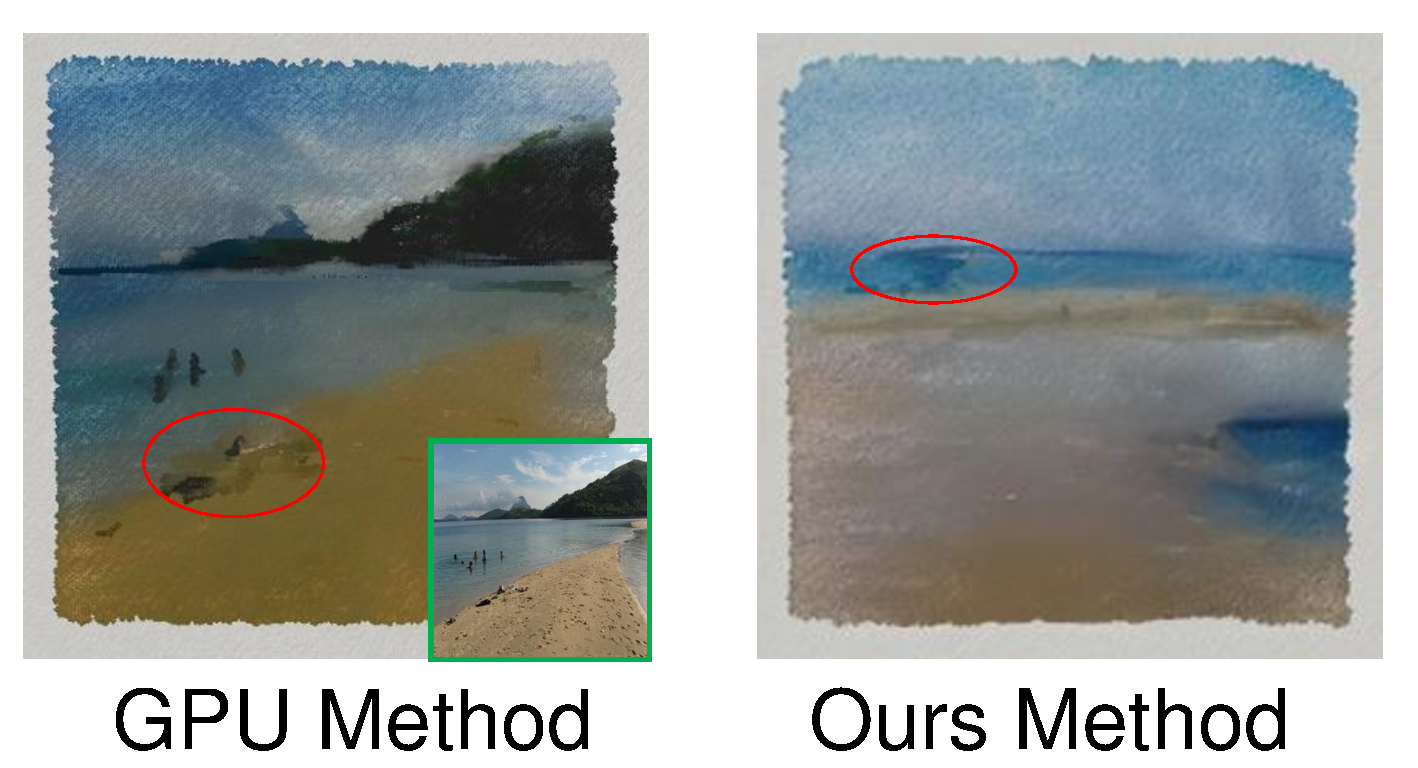
\includegraphics[width=7cm]{image/wGPU.pdf}
    \caption{Comparison of the generated image with GPU generation method(Sandbank)}
    \label{fig:wGPU}
\end{figure}

\subsection{Comparison with GPU method}
In the previous section, a GPU method was used to generate the dataset \cite{huang2021gpu}. A comparison of the generated images was carried out. The image style conversion by GPU method(green box is original image). and generated images with using the model in this paper. Approximate images were generated for ease of comparison(Sandbank image). As shown in Figure \ref{fig:wGPU}, the generation of the model in this paper well simulates the characteristics of watercolor images such as color blending (red circles), edge blurring (image edges), texture effects, etc., and the color transitions are soft, with good reconstruction of the dataset images.
\begin{figure}[h]
    \centering
    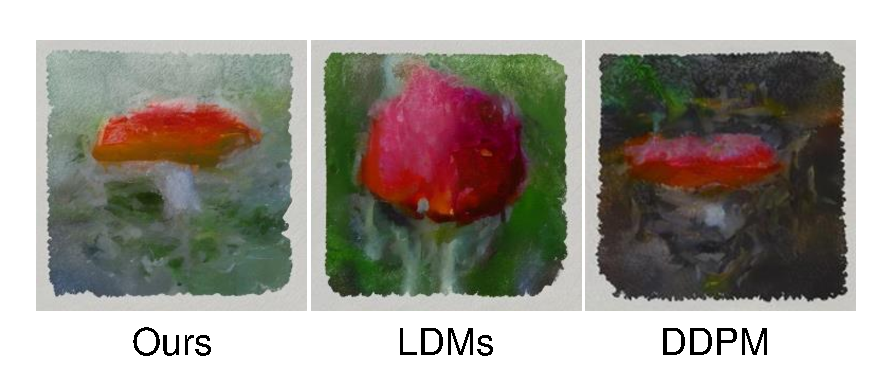
\includegraphics[width=8cm]{image/eva.pdf}
    \caption{Comparison of the generated image(Mushroom)}
    \label{fig:eva}
\end{figure}

\subsection{Evaluation}
In order to compare with the existing studies, the generated results of the model were objectively evaluated using FID \cite{FID}. As shown in Table \ref{tab:fid}, the model in this paper obtained the lowest FID compared to the original DDPM \cite{ho2020denoising} and LDMs \cite{rombach2022high}.
\begin{table}[htbp]
  \centering
  \caption{Objective evaluation}
  \label{tab:fid}
  \begin{tabular}{c c}
    \hline
    Model & FID  \\
    \hline
    DDPM & 55.632  \\
    LDMs & 47.263  \\
    Ours & 43.532  \\
    \hline
  \end{tabular}
\end{table}

Comparing the above three models generates images (mushrooms) as shown in Figure \ref{fig:eva}. The model in this paper achieved the best watercolor simulation subjectively. Looking closely at the generation results, this paper's model has a better reconstruction of the target within the image, and the unique features of watercolor images such as color diffusion and color fusion appear at the line edges of the image. Moreover, the generated image has fewer meaningless lines and color blocks and shows light and shadow effects to some extent.To further test the effectiveness of the model in this paper, more kinds of images were generated, as shown in Figure \ref{fig:eva1}.

\section{Conclusion}
In this study, a diffusion model for watercolor generation based on the Transformer structure is proposed. Experiments show that the model with this structure can improve the quality of watercolor image generation, proving the feasibility of this structure for the generation task, which can be extended to other generation tasks in the future. However, at present, the model may still have problems such as confusing lines in the face of complex scenes, which will be the next improvement goal to continue to improve the model performance.


%%%  参考文献 (Thebibliography)   %%%
\bibliographystyle{IEEEtran}
\bibliography{sample}

\end{document}
